% Copyright (C) 2012 Frederik Heber
% 
% This file is part of ScaFaCoS.
% 
% ScaFaCoS is free software: you can redistribute it and/or modify it
% under the terms of the GNU Lesser Public License as published by the
% Free Software Foundation, either version 3 of the License, or (at
% your option) any later version.
% 
% ScaFaCoS is distributed in the hope that it will be useful, but
% WITHOUT ANY WARRANTY; without even the implied warranty of
% MERCHANTABILITY or FITNESS FOR A PARTICULAR PURPOSE. See the GNU
% Lesser Public License for more details.
% 
% You should have received a copy of the GNU Lesser Public License
% along with this program. If not, see
% <http://www.gnu.org/licenses/>.
% 
%
% This is an illustration of the splitting of the Coulomb interactions into a
% short- and a long-range part. It has been created with TikZ and is modelled
% after an illustration in [Griebel, Knapek, Zumbusch - "Numerical Simulation 
% in Molecular Dynamics -- Numerics, Algorithms, Parallelization,
% Applications", 2007]
%
% Note that gnuplot is required to create the exponential peaks. Please refer
% to the documentation of TikZ.
%
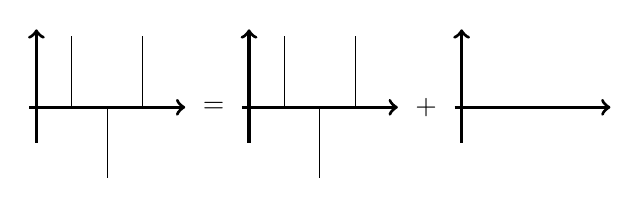
\begin{tikzpicture}[
	scale=0.9,
	axis/.style={very thick, ->},
]
   % axis
    \draw[axis] (-0.1,0)  -- (2.1,0);
    \draw[axis] (0,-0.5) -- (0,1.1);
	% peaks
	\draw (0.5,0) -- (0.5,1);
	\draw (1.,0) -- (1.,-1.);
	\draw (1.5,0) -- (1.5,1);

% equals
\node (equality) at (2.5,0) {=};

   % axis
    \draw[axis] (2.9,0)  -- (5.1,0);
    \draw[axis] (3,-0.5) -- (3,1.1);
	% peaks
	\draw (3.5,0) -- (3.5,1);
	\draw (4.,0) -- (4.,-1.);
	\draw (4.5,0) -- (4.5,1);
	% shields
	\draw[domain={3:4},samples=200,color=blue,dashed] plot[id=peak] function{-1*exp(-20*(x-3.5)**2)};
	\draw[domain={3.5:4.5},samples=200,color=blue,dashed] plot[id=peak] function{1*exp(-20*(x-4)**2)};
	\draw[domain={4:5},samples=200,color=blue,dashed] plot[id=peak] function{-1*exp(-20*(x-4.5)**2)};

% plus
\node (plus) at (5.5,0) {+};

   % axis
    \draw[axis] (5.9,0)  -- (8.1,0);
    \draw[axis] (6,-0.5) -- (6,1.1);
	% shields
	\draw[domain={6:7},samples=200,color=blue,dashed] plot[id=peak] function{1*exp(-20*(x-6.5)**2)};
	\draw[domain={6.5:7.5},samples=200,color=blue,dashed] plot[id=peak] function{-1*exp(-20*(x-7)**2)};
	\draw[domain={7:8},samples=200,color=blue,dashed] plot[id=peak] function{1*exp(-20*(x-7.5)**2)};

\end{tikzpicture}
